\documentclass{article} % For LaTeX2e


\usepackage{booktabs}
\usepackage[pdftex]{graphicx}
\usepackage{url}
\usepackage{multirow}
\usepackage{rotating} % For having vertical text in the tables.
\usepackage{wrapfig}

\usepackage{nips/nips11submit_e,times}


\title{Music Genre Classification}


\author{
Michael Haggblade \\
\And
Yang Hong \\
\And
Kenny Kao
}

\newcommand{\fix}{\marginpar{FIX}}
\newcommand{\new}{\marginpar{NEW}}

\nipsfinalcopy % Uncomment for camera-ready version

\begin{document}


\maketitle


\section{Introduction}
Music classification is an interesting problem with many applications, from Drinkify (a program that generates cocktails to match the music) to Pandora to dynamically generating images that complement the music. However, music genre classification has been a challenging task in the field of music information retrieval (MIR). Music genres are hard to systematically and consistently describe due to their inherent subjective nature.

In this paper, we investigate various machine learning algorithms, including k-nearest neighbor (k-NN), k-means, multi-class SVM, and neural networks to classify the following four genres: classical, jazz, metal, and pop. We relied purely on Mel Frequency Cepstral Coefficients (MFCC) to characterize our data as recommended by previous work in this field \cite{MFCC, General}. We then applied the machine learning algorithms using the MFCCs as our features. 



\section{Our Approach}

\subsection{Data Retrieval Process}

\input{text/data_retrieval_process.tex}

\subsection{Mel Frequency Cepstral Coefficients (MFCC)}

\input{text/mfcc.tex}

\begin{figure}[!hb]
  \centering
  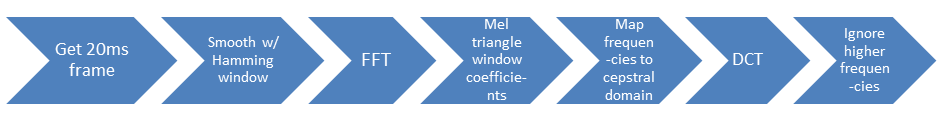
\includegraphics[width=.88\textwidth]{images/our_approach-mfcc_flow.png}
  \caption{MFCC Flow}
  \label{fig:mfcc_flow}
\end{figure}


\section{Techniques}

\subsection{Kullback-Lieber (KL) Divergence}

\input{text/kldiv1.tex}

\begin{figure}[!hb]
  \centering
  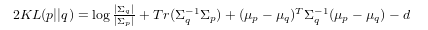
\includegraphics[width=.88\textwidth]{images/techniques-kldiv-kleqn.png}
\end{figure}

\input{text/kldiv2.tex}

\begin{figure}[!hb]
  \centering
  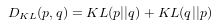
\includegraphics[width=.38\textwidth]{images/techniques-kldiv-dkleqn.png}
\end{figure}

\subsection{k-Nearest Neighbors (k-NN)}

\input{text/knn.tex}

\subsection{k-Means}

\input{text/kmeans.tex}

\subsection{Multi-Class Support Vector Machine (DAG SVM)}

\begin{minipage}{.5\textwidth}\centering
%\begin{wrapfigure}{r}{0.5\textwidth}
%\begin{figure}
  %\centering
  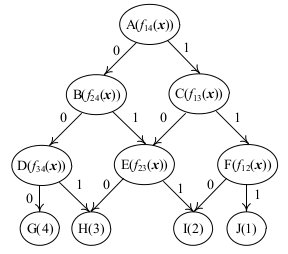
\includegraphics[width=.58\textwidth]{images/techniques-dag-example.png}

  A directed acyclic graph of 2-class SVMs
  %\caption{A directed acyclic graph of 2-class SVMs}
%\end{figure}
%\end{wrapfigure}
\end{minipage}
\begin{minipage}{.5\textwidth}%\centering
SVM classifiers provide a reliable and fast way to differentiate between data with only two classes. In order to generalize SVMs to data falling into multiple classes (i.e. genres) we use a directed acyclic graph (DAG) of two-class SVMs trained on each pair of classes in our data set (eg $f_{14}(x)$ denotes the regular SVM trained on class 1 vs class 4) \cite{dag}. We then evaluate a sequence of two-class SVMs and use a process of elimination to determine the output of our multi-class classifier.

\end{minipage}


\subsection{Neural Networks}

We tried neural networks because it has proved generally successful in many machine learning problems.
We first pre-process the input data by combining the mean vector and the top half of the covariance matrix (since it is symmetric) into one feature vector. 
As a result, we get $15 + (1+15)*\frac{15}{2}$ features for each song. 
We then process the output data by assigning each genre to an element in the set of the standard orthonormal basis in $R^4$ for our four genres, as shown in the table below:


\begin{center}
\begin{tabular}{| c | c | c | c | c |}
\hline
Genre & Classical & Jazz & Metal & Pop \\
\hline
Vector & (1, 0, 0, 0) & (0, 1, 0, 0) & (0, 0, 1, 1) & (0, 0, 0, 1) \\
\hline
\end{tabular}
\end{center}

\input{text/nn2.tex}


\section{Results}

% SVM and NN Results tables
\begin{table}[!ht]

\begin{minipage}{.5\textwidth}\centering
\caption{DAG SVM Results}
\begin{tabular}{| c c | c c c c |}
%\toprule
\hline
& & \multicolumn{4}{| c |}{Actual} \\
& & Classical & Jazz & Metal & Pop \\
\hline
\multirow{4}{*}{\begin{sideways}Predicted\end{sideways}}
& Classical & 29 & 4 & 1 & 1 \\
& Jazz & 1 & 20 & 1 & 0 \\
& Metal & 0 & 4 & 26 & 0 \\
& Pop & 0 & 2 & 2 & 29 \\
%\bottomrule
\hline
\multicolumn{2}{| c |}{Accuracy} & 97\% & 67\% & 87\% & 97\% \\
\hline
\end{tabular}
\end{minipage}
\hspace{.5cm}
\begin{minipage}{.5\textwidth}\centering
\caption{Neural Network Results}
\begin{tabular}{| c c | c c c c |}
%\toprule
\hline
& & \multicolumn{4}{| c |}{Actual} \\
& & Classical & Jazz & Metal & Pop \\
\hline
\multirow{4}{*}{\begin{sideways}Predicted\end{sideways}}
& Classical & 14 & 0 & 0 & 0 \\
& Jazz & 1 & 12 & 4 & 0 \\
& Metal & 0 & 0 & 13 & 0 \\
& Pop & 1 & 0 & 0 & 19 \\
%\bottomrule
\hline
\multicolumn{2}{| c |}{Accuracy} & 88\% & 100\% & 76\% & 100\% \\
\hline
\end{tabular}
\end{minipage}

\end{table}

% kmeans and kNN Results tables
\begin{table}[!ht]

\begin{minipage}{.5\textwidth}\centering
\caption{k-Means Results}
\begin{tabular}{| c c | c c c c |}
%\toprule
\hline
& & \multicolumn{4}{| c |}{Actual} \\
& & Classical & Jazz & Metal & Pop \\
\hline
\multirow{4}{*}{\begin{sideways}Predicted\end{sideways}}
& Classical & 14 & 16 & 0 & 0 \\
& Jazz & 2 & 27 & 1 & 0 \\
& Metal & 0 & 0 & 27 & 3 \\
& Pop & 0 & 1 & 1 & 28 \\
%\bottomrule
\hline
\multicolumn{2}{| c |}{Accuracy} & 88\% & 61\% & 93\% & 90\% \\
\hline
\end{tabular}
\end{minipage}
\hspace{.5cm}
\begin{minipage}{.5\textwidth}\centering
\caption{k-NN Results}
\begin{tabular}{| c c | c c c c |}
%\toprule
\hline
& & \multicolumn{4}{| c |}{Actual} \\
& & Classical & Jazz & Metal & Pop \\
\hline
\multirow{4}{*}{\begin{sideways}Predicted\end{sideways}}
& Classical & 26 & 9 & 0 & 2 \\
& Jazz & 4 & 20 & 4 & 1 \\
& Metal & 0 & 1 & 24 & 0 \\
& Pop & 0 & 0 & 2 & 27 \\
%\bottomrule
\hline
\multicolumn{2}{| c |}{Accuracy} & 87\% & 67\% & 80\% & 90\% \\
\hline
\end{tabular}
\end{minipage}

\end{table}

Classification accuracy varied between the different machine learning techniques and genres. The SVM had a success rate of only 66\% when identifying jazz , most frequently misidentifying it as classical or metal. The Neural Network did worst when identifying metal with a 76\% success rate. Interestingly, the Neural Network only ever misidentified metal as jazz. k-Means did well identifying all genres but Jazz, which was confused with Classical 36\% of the time. k-NN had difficulty differentiating between Metal and Jazz in both directions. Of its 33\% failures identifying Jazz, it misidentifies as Metal 90\% of the time. Similarly, k-NN incorrectly predicted that Metal songs would be Jazz in 66\% of all its failed Metal identifications.

Overall we found that k-NN and k-means yielded similar accuracies of about 80\%. A DAG SVM gave about 87\% accuracy and neural networks gave 96\% accuracy.



\section{Conclusion}

\subsection{Discussion}

\input{text/discussion.tex}

\subsection{Future Work}

\input{text/future_work.tex}


\begin{thebibliography}{9}
\bibitem{dag}
  \emph{Chen, P., Liu, S.}.
  "An Improved DAG-SVM for Multi-class Classification"
  \url{http://ieeexplore.ieee.org/stamp/stamp.jsp?arnumber=0566976}.

\bibitem{marsyas}
  \emph{Marsyas}.
  "Data Sets"
  \url{http://marsysas.info/download/data\_sets}.

\bibitem{kldiv}
  \emph{Mandel, M., Ellis, D.}.
  "Song-Level Features and SVMs for Music Classification"
  \url{http://www.ee.columbia.edu/~dpwe/pubs/ismir05-svm.pdf}.

\bibitem{nn}
  \emph{Li, T., Chan, A., Chun, A.}.
  "Automatic Musical Pattern Feature Extraction Using Convolutional Neural Network."
  IMECS 2010.
  \url{http://www.iaeng.org/publication/IMECS2010/IMECS2010\_pp546-550.pdf}.

\bibitem{general}
  \emph{Fu, A., Lu, G., Ting, K.M., Zhang, D.}.
  "A Survey of Audio-Based Music Classification and Annotation"
  IEEE Transactions on Multimedia.
  \url{http://ieeexplore.ieee.org/stamp/stamp.jsp?tp=&arnumber=5664796&tag=1}.

\end{thebibliography}

\end{document}
